\documentclass[border=12pt]{standalone}
\usepackage{amsmath, amssymb}
\usepackage{tikz}
\definecolor{ring0}{HTML}{0033CC}
\definecolor{ring1}{HTML}{0066FF}
\definecolor{ring2}{HTML}{0099FF}
\definecolor{ring3}{HTML}{00CCCC}
\definecolor{ring4}{HTML}{00CC66}
\definecolor{ring5}{HTML}{33CC00}
\definecolor{ring6}{HTML}{99CC00}
\definecolor{ring7}{HTML}{CCCC00}
\definecolor{ring8}{HTML}{FF9900}
\definecolor{ring9}{HTML}{FF6600}
\definecolor{ring10}{HTML}{FF3300}
\definecolor{ring11}{HTML}{CC0000}
\definecolor{gap0}{HTML}{E53935}
\definecolor{gap1}{HTML}{1E88E5}
\definecolor{gapfar}{HTML}{CCCCCC}
\begin{document}
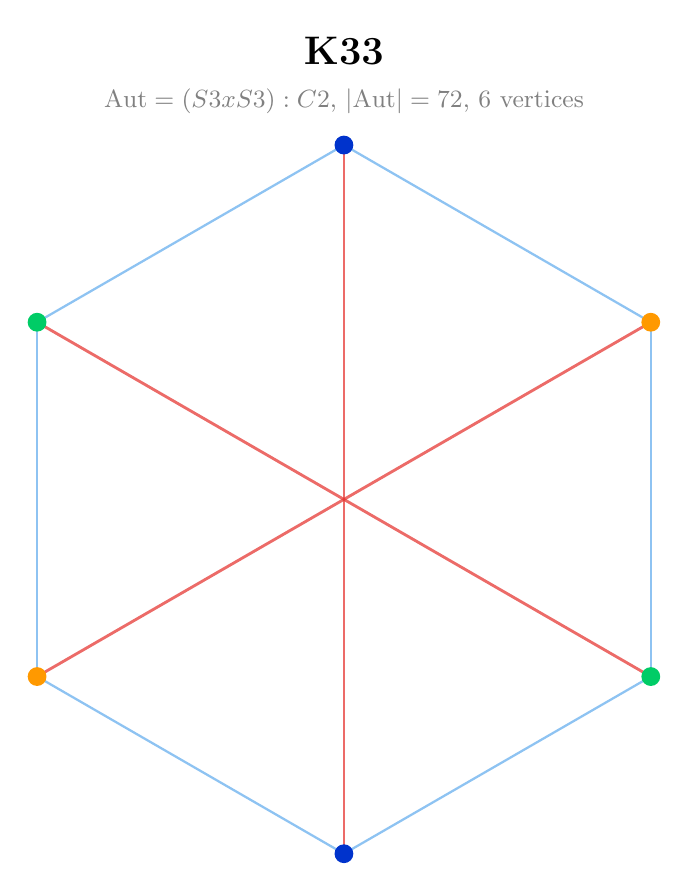
\begin{tikzpicture}
\node[font=\Large\bfseries] at (0, 5.70) {K33};
\node[font=\small, text=gray] at (0, 5.05) {$\mathrm{Aut} = (S3 x S3) : C2$, $|\mathrm{Aut}| = 72$, 6 vertices};
\draw[line width=0.82pt, gap1, opacity=0.50] (0.000, 4.500) -- (-3.897, 2.250);
\draw[line width=0.82pt, gap1, opacity=0.50] (0.000, 4.500) -- (3.897, 2.250);
\draw[line width=0.82pt, gap1, opacity=0.50] (3.897, -2.250) -- (-0.000, -4.500);
\draw[line width=0.82pt, gap1, opacity=0.50] (3.897, -2.250) -- (3.897, 2.250);
\draw[line width=0.82pt, gap1, opacity=0.50] (-3.897, -2.250) -- (-0.000, -4.500);
\draw[line width=0.82pt, gap1, opacity=0.50] (-3.897, -2.250) -- (-3.897, 2.250);
\draw[line width=1.03pt, gap0, opacity=0.75] (0.000, 4.500) -- (-0.000, -4.500);
\draw[line width=1.03pt, gap0, opacity=0.75] (3.897, -2.250) -- (-3.897, 2.250);
\draw[line width=1.03pt, gap0, opacity=0.75] (-3.897, -2.250) -- (3.897, 2.250);
\fill[ring0] (0.000, 4.500) circle (3.4pt);
\fill[ring4] (3.897, -2.250) circle (3.4pt);
\fill[ring8] (-3.897, -2.250) circle (3.4pt);
\fill[ring0] (-0.000, -4.500) circle (3.4pt);
\fill[ring4] (-3.897, 2.250) circle (3.4pt);
\fill[ring8] (3.897, 2.250) circle (3.4pt);
\end{tikzpicture}
\end{document}